\section{Appendix C-Koenigs: conjugacy details and exceptional cases}
\label{app:c-koenigs}

This appendix supports Section~\ref{sec:ap-koenigs}. It records the affine conjugacy between the logistic and quadratic families, the Becker--Bergweiler dichotomy, the elementary solutions at $r=2$ and $r=4$, and domain remarks for the identity $A(p)=2\phi_{2p}(\tfrac12)$.

\subsection{Affine conjugacy to $z^2+c$}

\begin{lemma}
\label{lem:logistic-quadratic}
The logistic map $f_r(x)=r x(1-x)$ is affinely conjugate to $P_c(z)=z^2+c$ with
\begin{equation}
\label{eq:c-of-r}
c(r)
=
\frac{2r-r^2}{4}.
\end{equation}
\end{lemma}

\begin{proof}[Proof sketch]
Seek $h(x)=ax+b$ with $h\circ f_r\circ h^{-1}=P_c$. The standard choice $x=-\frac{z}{r}+\frac12$ (for $r\neq 0$) conjugates $f_r$ to a monic quadratic $z^2+c$; matching coefficients yields \eqref{eq:c-of-r}.
\end{proof}

Under $r\in(0,1)$ one has $c(r)\in\bigl(0,\tfrac14\bigr)$. The exceptional integrable quadratics below correspond to $c=0$ ($r=2$) and $c=-2$ ($r=4$), both outside $\bigl(0,\tfrac14\bigr)$.

\begin{figure}[ht]
\centering
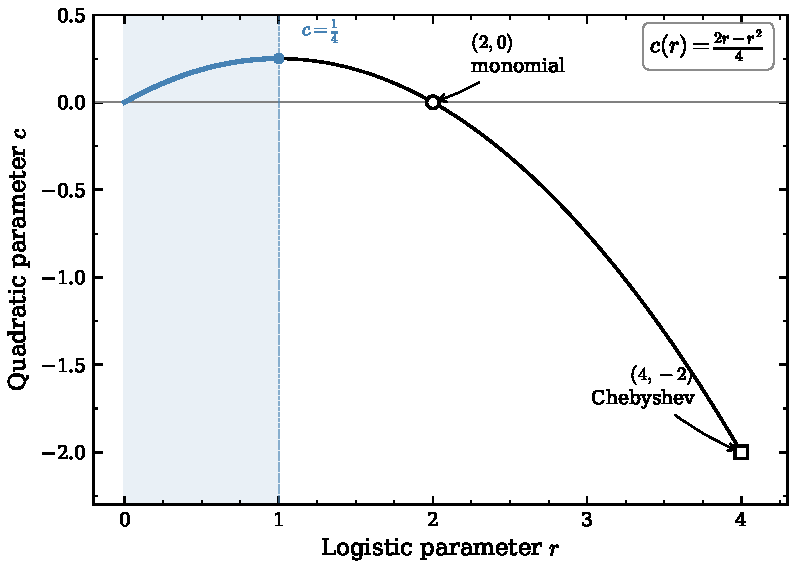
\includegraphics[width=0.7\textwidth]{figures/fig_ap_koenigs/figure1_parameter_conjugacy.pdf}
\caption{Parameter correspondence $c(r)=(2r-r^2)/4$. The segment $r\in(0,1)$ maps to $c\in(0,\tfrac14)$, disjoint from the integrable values $c\in\{0,-2\}$.}
\label{fig:c-of-r}
\end{figure}

\subsection{Non-elementarity for multipliers in $(0,1)$}

For $r\in(0,1)$ the origin is an attracting fixed point of $f_r$ with multiplier $\lambda=r\in(0,1)$, and classical linearisation (Koenigs) supplies a holomorphic conjugacy $\phi_r$ near $0$ satisfying \eqref{eq:schroder}. Results of Becker and Bergweiler on hypertranscendence of conjugacies in complex dynamics \cite{Becker1995} imply that, for rational maps of degree at least two, such linearisations are differentially algebraic only in highly exceptional normal forms (monomial / Chebyshev type). Under the conjugacy of Lemma~\ref{lem:logistic-quadratic}, the interval $r\in(0,1)$ maps to $c\in\bigl(0,\tfrac14\bigr)$, which avoids those exceptional quadratic parameters. Hence for each fixed $r\in(0,1)$ the conjugacy $\phi_r$ is non-elementary as a function of $z$.

\begin{remark}[Solvable logistic parameters outside the branching range]
\label{rem:r2r4}
The logistic parameters $r=2$ and $r=4$ are classically solvable (logarithmic and inverse-trigonometric linearisations, up to normalisation), corresponding under \eqref{eq:c-of-r} to $c=0$ and $c=-2$. At those parameters the multiplier at $0$ is \emph{repelling} ($|r|>1$), so the linearisation is of Poincar\'e rather than attracting-Koenigs type. They illustrate that elementary formulae exist only for exceptional multipliers \emph{outside} $r\in(0,1)$; they are not counter-examples inside the subcritical branching window $r=2p\in[0,1)$.
\end{remark}

\subsection{Elementary displays at $r=2$ and $r=4$ (outside Path~C range)}

\paragraph{Case $r=2$ ($c=0$).}
A standard normalisation yields a logarithmic linearisation equivalent to $-\tfrac12\log(1-2z)$ on a suitable domain.

\paragraph{Case $r=4$ ($c=-2$).}
A standard normalisation is proportional to $(\arcsin\sqrt{z})^2$.

Neither formula supplies an elementary closed form for general $r\in(0,1)$.

\subsection{On $A(p)=2\phi_{2p}(\tfrac12)$}

With $w_{n+1}=f_r(w_n)$, $r=2p$, $w_0=\tfrac12$, the Koenigs limit \eqref{eq:koenigs-limit} gives
\[
\phi_r\bigl(\tfrac12\bigr)
=
\lim_{n\to\infty}
r^{-n} f_r^{\circ n}\bigl(\tfrac12\bigr)
=
\lim_{n\to\infty}
\frac{w_n}{r^n},
\]
whenever the orbit stays in the domain where the limit representation holds. For $r\in(0,1)$ the origin is attracting on the real line and $w_0=\tfrac12$ iterates towards $0$ under $f_r$, so the real orbit is the natural candidate for the limit. Then
\[
A(p)
=
2\lim_{n\to\infty}\frac{w_n}{r^n}
=
2\phi_r\bigl(\tfrac12\bigr)
\]
as stated in \eqref{eq:Ap-koenigs}. The endpoint $p=0$ ($r=0$) is elementary and degenerate (immediate extinction after the first generation in the binary model with $p=0$); it may be checked directly that $A(0)=\tfrac12$ matches $\tfrac12\prod_{k\geq 1}(1-w_k)$ with $w_k=0$ for $k\geq 1$ after the first step, consistently with $A(p)\leq\tfrac12$.

\subsection{Parameter-dependent versus fixed-$r$ statements}

Fixed-$r$ non-elementarity constrains $\phi_r$ as a function of $z$, whereas the thesis uses the scalar $A(p)=2\phi_{2p}(\tfrac12)$. Even for a single $r$, non-elementarity of $z\mapsto\phi_r(z)$ does not by itself forbid a closed form for one value $\phi_r(\tfrac12)$; and elevating the statement to a classification of $p\mapsto A(p)$ is a further step. The main text therefore adopts the careful claim quoted in Section~\ref{sec:no-elementary}.
